In your master studies you are relatively free in how you compile your timetable. However, it is important that you cover your optional areas of courses with ECTS credits. 
%The following table shows in the first column the area of studies, in the second column your choices out of that area which you can attend, in the third column the recommended semester to hear this lecture and in the fourth column the awarded ECTS.\\
The following tables show some examples of choices for courses you can make, depending on which direction you want to focus:\\

\begin{center}
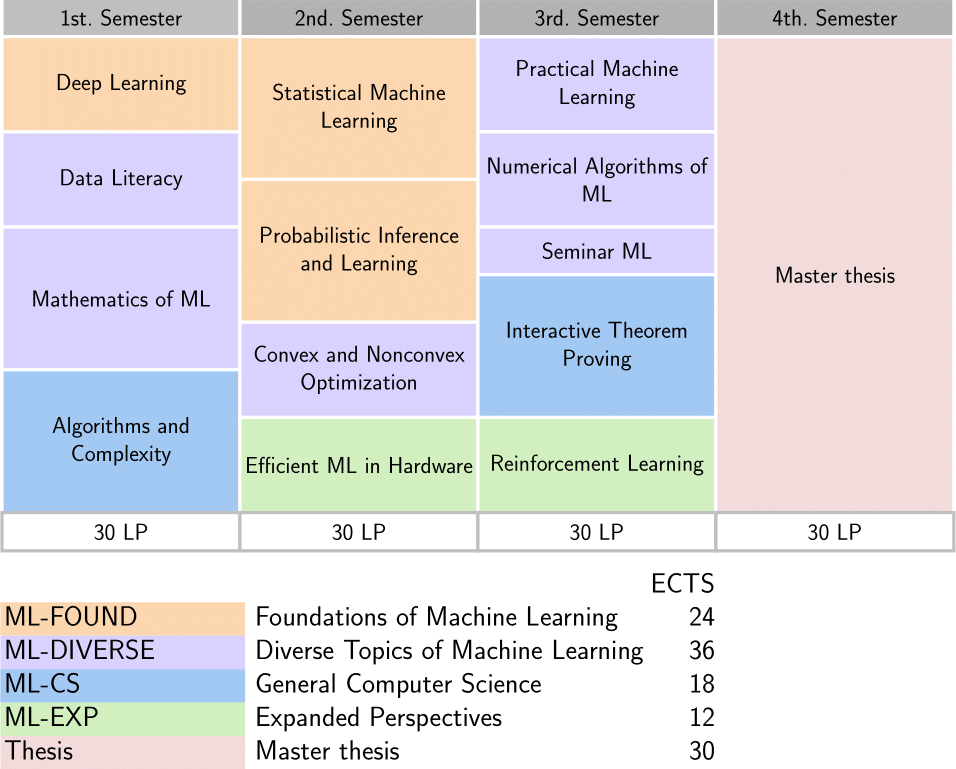
\includegraphics[scale=0.65]{media/ML_Theorie}~\\
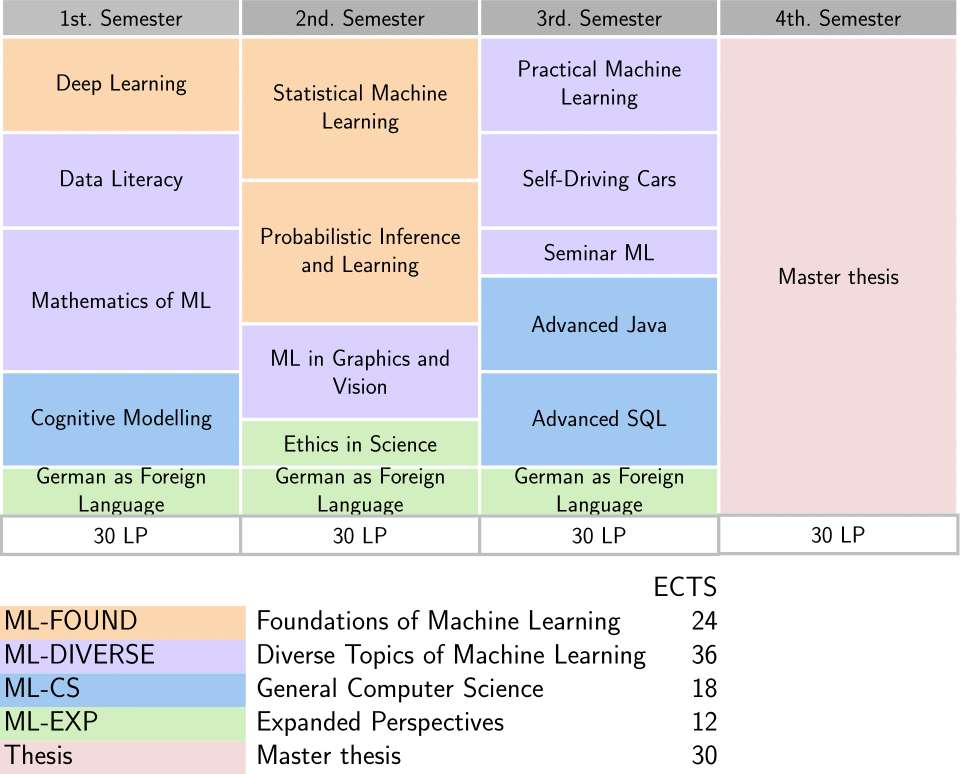
\includegraphics[scale=0.65]{media/ML_Praktisch}~\\
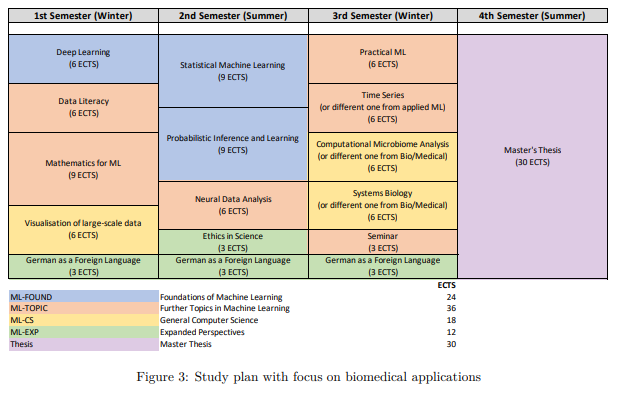
\includegraphics[scale=0.65]{media/ML_Biomed}~\\
\end{center}

All three lectures out of \emph{Foundations of Machine Learning} are mandatory, you need 24 ECTS. Out of \emph{Diverse Topics in Machine Learning} you need 36 ECTS, of which no more than 6 ECTS can be from seminars and no more than 6 ECTS can be from practical ML. The areas \emph{General Computer Science} and \emph{Expanded Perspectives} are special. Here, you can attend any graded lecture out of Computer Science (for General Computer Science) or any graded lecture out
of all the offered lectures in the whole university, except university sports (for Expanded Perspectives) for a total of 18 ECTS and 12 ECTS respectively.
Further Information can be found in your module handbook at:\\
\url{https://uni-tuebingen.de/de/135400}
